\documentclass{article}
\usepackage{amsmath, amssymb, graphics}
\usepackage{subfig}
\usepackage{graphicx}\usepackage{graphicx}
\begin{document}

\title{An Alternative Approach of the Analytic Moment of Fluid Reconstruction in 2D}
\author{Zhouteng Ye}

\maketitle

The MOF reconstruction uses the information of both centroid and volume to obtains the approximate linear reconstruction of the interface in 2D.
In the original Moment of Fluid (MOF) paper and the analytic MOF paper, 
when a reference centroid $\bf{x}_0$ and volume $V_0$ is given, 
they both minimize the Euclidian distance from the reference centroid and the reconstruction centroid

\begin{equation}
\rm{min}\|\bf{x-x_0}\|
\end{equation}

In this study, a new non-Euclidian distance is used to minimize the distance between the reference centroid and the reconstruction centroid. 
In 2D case, for a given volume $V_0 \in (0,1)$, all possible location of the centroids with linear reconstruction is a continuous and closed curve.
The surface and contour lines for the function $V = f(x,y)$ is plotted in Figure 1.

Let 
\begin{equation}
ax+by+c=0
\end{equation}
the reconstruction straight line. 
The corresponding centroid is $(p_x,p_y)$ and the volume is $V=f(\bf{p_x,p_y})$.
An important properity of the contour lines is the tangent vector of the contour line is perpendicular to the reconstruction interface
\begin{equation}
\nabla V \cdot (-a,b) = 0
\end{equation}

For any points on the $V = f(x,y)$ , the line with a given normal vector on the surface is perpendicular to the corresponding contour line. 
The projection of the contour lines and constant normal lines are shown in Figure 1(b), 
where the solid line represents the constant volume line and dashed lien indicates the constant normal vector line.
Solid lines and dashed lines are perpendicular with each other on the 3-D surface $V = f(x,y)$, 
but not perpendicular with each other on the projection plain.

The shortest path from the reference centroid $(x_0,y_0)$ to the contour of reference volume $V_0$ is to travel along its corresponding constant normal line (das line in Figure 1(b)) until it reaches the contour value $V_0$. 
In 2D, all contour lines and constan normal lines have analytic form, 
it is easy to find the intersection of the corresponding contour line and constan normal line.

The main purpose is to comparison of the reconstruction accuracy and efficiency between the traditional Euclidian distance and the proposed non-Euclidian distance apporach. 
The non-Euclidian distance apporach can also work with the numerical approach in the further work, 
the properity of the surface makes it easy to find out the normal vector of the reconstruction instead of iteration approach.


\begin{figure}[h]
\centering

\subfloat[surface and contourlines of the function $V=f(x,y)$]{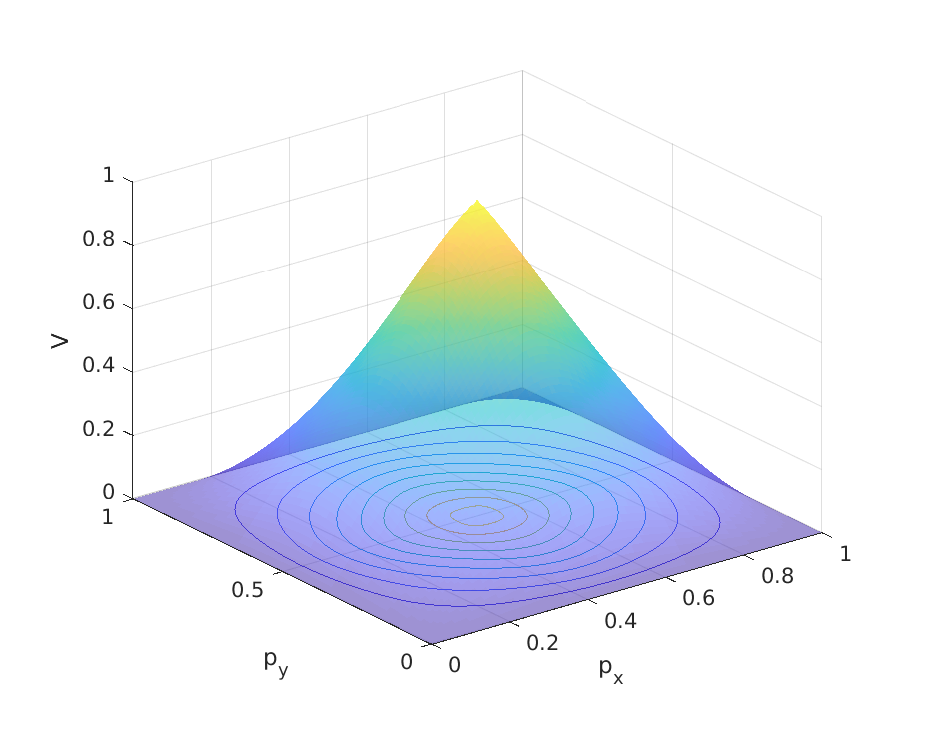
\includegraphics[width = 0.48\textwidth]{Manifold_surface.eps}}
\subfloat[Constant Volume contour lines and constant normal vector line.]{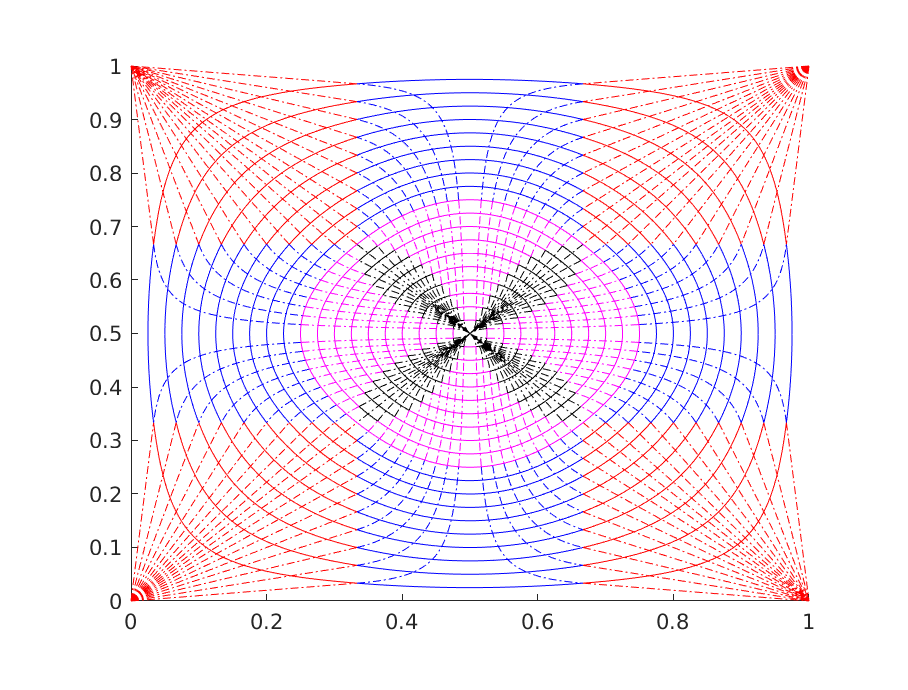
\includegraphics[width = 0.48\textwidth]{mainfold_projection.eps}}

\caption{Figures for the function }

\end{figure}

\section*{reference}

[1] Dyadechko, V. and Shashkov, M., 2005. Moment-of-fluid interface reconstruction. Los Alamos Report LA-UR-05-7571.

[2] Lemoine, A., Glockner, S. and Breil, J., 2017. Moment-of-fluid analytic reconstruction on 2D Cartesian grids. Journal of Computational Physics, 328, pp.131-139.

\end{document}